\documentclass{article}

% --- NeurIPS 2026 TAE workshop style -------------------------------------
% neurips_2026.sty is vendored at paper/template/neurips_2026.sty and is
% copied next to this .tex by build.py on every run (see ensure_style_file),
% so a fresh checkout compiles without a manual download step.
%
% Style option list is driven by the CAMERA_READY constant above this
% template string. SUBMISSION mode (CAMERA_READY=False, per DECISION.md
% Section 1) loads plain [dblblindworkshop]. Camera-ready mode
% (CAMERA_READY=True) loads [dblblindworkshop, final] -- the "final" option
% is what de-anonymises the paper, so it must NOT be added until the paper
% is accepted and ANONYMITY.md's de-anonymisation step is deliberately taken.
\usepackage[dblblindworkshop]{neurips_2026}

\usepackage[utf8]{inputenc}
\usepackage[T1]{fontenc}
\usepackage{graphicx}
\usepackage{booktabs}
\usepackage{amsmath}
\usepackage{hyperref}

% TYPE 3 FONT FIX, 2026-08-03. template/neurips_2026.tex:376-378 requires
% "only Type 1 or Embedded TrueType fonts" and :416-417 warns that a Type 3
% font will be sent back to be fixed. With [T1]{fontenc} loaded and no Type 1
% T1 typewriter family installed, MiKTeX silently fell back to the METAFONT
% bitmap ectt1000.pk at 600 dpi and embedded it as a Type 3 font on page 1 --
% the five glyphs a/e/i/l/m spelling the \texttt{email} line inside the .sty's
% own anonymous author block (neurips_2026.sty:341). Mapping the typewriter
% family to Courier (pcr, a Type 1 face from psnfss) removes it.
%
% Do NOT "fix" this with \usepackage{lmodern}: that also resets \rmdefault and
% would override the style file's \rmdefault=ptm (neurips_2026.sty:101-102),
% changing the body font away from Times. This line touches \ttdefault ONLY,
% so \rmdefault=ptm and \sfdefault=phv are left exactly as the .sty sets them.
\renewcommand{\ttdefault}{pcr}

% Figure blocks below give the path recorded in manuscript.md relative to
% SUBMISSION_2026/TAE/ (e.g. "figures/fig1_rule_layers.pdf"); this compile
% happens from SUBMISSION_2026/TAE/paper/, one level under that, so the
% search path is the sibling figures/ directory, and \includegraphics below
% is called with just the basename.
\graphicspath{{../figures/}}

% Unresolved-number markers stay visually obvious rather than silently
% compiling as blank groups -- see substitute.py for the resolution step.
\newcommand{\claimplaceholder}[1]{\texttt{\{\{CLAIM:#1\}\}}}

\title{When Guardrails Change What Gets Counted: Conformance Metrics with Agent-Reported Rule Conditions}

% dblblindworkshop mode requires \workshoptitle{} IN ADDITION TO \title{}
% (template/neurips_2026.tex:41-43). The two are not interchangeable: the
% .sty consumes \workshoptitle only inside \@trackname, which typesets the
% first-page footnote "...(NeurIPS 2026). Workshop: <workshoptitle>."
% (neurips_2026.sty:81-92). It therefore holds the WORKSHOP's name, not the
% paper's -- setting it to the paper title prints the paper title in the
% venue footnote, which is wrong and was the state before 2026-08-01.
%
% Do not expect to see it in the submission PDF. \@trackname is expanded
% only under \if@neuripsfinal (neurips_2026.sty:396-398); without "final"
% the footnote is the generic "Submitted to 40th Conference ... Do not
% distribute." This line is silent now and correct at camera-ready.
\workshoptitle{TAE (Trust-AI-Eval): Can We Trust AI Evaluation?}

% Double-blind: no \author{} content until de-anonymisation.
\author{}

\begin{document}

\maketitle

\begin{abstract}
Runtime guardrails check proposed actions and ask an agent to retry when a rule is violated. Evaluations often use a conformance rate: the share of decisions that satisfy a rule. That rate is difficult to interpret when the condition is written by the agent in the response being judged. Blocking a response can change the final action and which decisions satisfy its condition. This does not require deception. Some rules read an agent-reported condition, while others read simulator-recorded state. We compare paired runs with and without validators across nine model configurations in two agent testbeds.

The primary rate counts demand increases among decisions reporting high scarcity; we call it the conditional increase rate. This group includes the full high-scarcity/high-coping condition, but also decisions with low coping. In the anchor configuration, the no-validator-minus-validator contrast is +45.73 pp for high-scarcity prevalence and +23.02 pp for the conditional increase rate. A descriptive reweighting to a common simulator-recorded world-state distribution leaves $-$2.53 pp at 100\% coverage and +0.21 pp at the finest stratification. Because that world state is downstream of enforcement, this is not a causal adjustment. It is consistent with a large composition contribution, but does not rule out a within-world reporting effect.

On gemma3:12b, the conditional gain +11.44 pp becomes +0.16 pp (95\% CI $-$13.92, +14.25; p = 0.965) when we use a design-fixed denominator on three seeds. Replacing the agent-reported condition with a world-state condition does not remove the feedback problem. We recommend reporting condition prevalence in both arms beside every conformance rate and logging the independent world state behind an agent report when it exists.

\end{abstract}
\section{Introduction}
Runtime guardrails can change the response that they later score. This matters for large language model (LLM) agents, which are often paired with runtime checks. We use \textit{validator} for the component that applies a rule, identifies a violation, and asks the agent to retry [1] [2] [3] [4]. A conformance rate is the share of decisions that pass the rule. A paired evaluation can compare that share with and without validators, but the comparison is meaningful only when the two arms count comparable decisions. The loop also builds on earlier work on machine-readable norms and agent institutions [5] [6] [7] [8]. The central problem is that the condition used to select decisions for the rate may itself be part of the agent's response. If enforcement changes that condition, a changed rate may reflect a changed set of counted decisions rather than changed behavior.

Consider an irrigation agent that proposes increasing water demand while reporting high water scarcity. A validator can block this response and ask for a retry. The retry may change both the action and the report. Here, an \textit{agent-reported condition} is a label written by the agent in the same response as the action. The validator reads that label to decide whether to block. The metric reads the same label to decide whether the decision enters the rate. If the evaluation counts increases only among decisions that report high scarcity, enforcement can change both the recorded action and the set of decisions counted by the rate. Figure 1 summarizes this path. We observe the recorded response, not the agent's hidden intent.

% figure source (as recorded in manuscript.md): figures/fig0_problem_schematic.pdf
\begin{figure}[t]
\centering
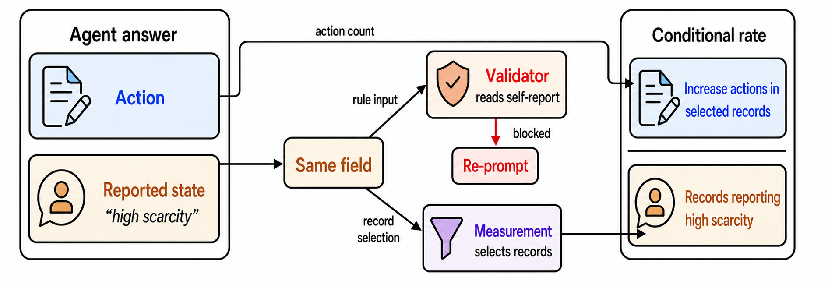
\includegraphics[width=0.8\linewidth]{fig0_problem_schematic.pdf}
\caption{How an agent-reported condition changes what a metric counts. One response contains an action and a reported condition. The validator reads the condition to decide whether to block. The metric reads the same condition to select decisions for the rate. A blocked response may be retried, producing a different recorded response. High scarcity is an illustrative irrigation label. This is a conceptual example, not a data figure.}
\label{fig:1}
\end{figure}

Prior work on LLM benchmarks and agent evaluation shows that scores can be hard to interpret when the measured construct or evaluation conditions change [12] [13] [14]. Here, enforcement can change the condition itself because the agent writes it in the response being evaluated.

The problem also relates to treatment-affected variables. In agentic code repair, a variable observed after an intervention can be affected by that intervention [9]. Causal-methods work therefore warns against treating such a variable as an independent control [10]. Some settings can address this issue by branching from a frozen external state. An agent-reported condition has no independent version outside the response being evaluated. Freezing the original report would remove the behavior that the rule is intended to evaluate.

We ask three questions. First, does enforcement change how often the agent reports the condition, as well as the rate computed among those reports? Second, how much of the change in the anchor configuration is descriptively associated with different simulator-recorded world states? Third, which additional statistics remain interpretable when a rate over every decision is available?

We make three contributions. First, we identify a construct-validity failure mode for runtime guardrail evaluation. When a rule condition is written by the agent, enforcement can change both the response and the set of responses used to score it. Second, we demonstrate this failure mode in paired simulations across two agent testbeds. We separate rules that read agent reports from rules that read simulator-recorded state. Third, we provide a reporting protocol. It pairs the conditional rate with condition prevalence, an independent world-state record, and a rate over every decision when the design allows it. Our claims are descriptive. We do not claim that agents deceive, that recorded-world reweighting is a causal adjustment, or that the pattern applies to every model or governance stack. Section 2 defines the guardrail loop and the paired simulation design.

\section{Experimental Setup}
Both testbeds run the same guardrail loop. In each generation, the agent returns an action and two agent-reported conditions about its situation. Validators check the proposal against those reports and against the simulator's recorded state. An ERROR-level violation returns the broken rule and asks for another answer, up to three attempts. If all attempts fail, a domain default executes.

The rule under study forbids an increase in demand when the agent reports both high water scarcity and high coping capacity. Both labels are written by the agent in the generation being judged. We call their combination the \textit{full conjunction}. We use the scarcity label as the primary conditioning variable. It is a \textit{marginal proxy}: it includes every decision satisfying the full conjunction, but also includes decisions with low coping. Table 1 reports the coping label and the full conjunction separately.

Irrigation is the primary testbed: 78 farm agents over 42 years and 3,276 decisions per run. It models scarcity and coping, uses five paired seeds in most cells, and has fewer seeds in two cells. It has five action types and a water right cap. A coupled reservoir makes one year's action change the next year's state. Flood uses Protection Motivation Theory [11] and four action types. It has no action-to-environment feedback, so it serves as a portability demonstration rather than a control for enforcement pressure.

The corpus holds nine model configurations from three open-weight model families spanning 3B to 27B. Each has validator-on and validator-off runs. All nine appear in flood and five in irrigation, giving fourteen model-testbed cells. The arms are paired within a cell. Most cells use five seeds; two irrigation cells use fewer. Table 1 reports the value of \textit{n}.

\section{Rule Inputs: Agent-Reported vs. World-Recorded}
Only some rules read the agent's report. A \textit{world state} is an environment condition recorded by the simulator, not a label written by the agent. World-feasibility rules use it, such as the water-right cap. Other rules use scarcity and coping labels written in the same response as the action. We separate these inputs before interpreting the conditional rate.

The corpus separates these layers in the anchor cell, which has five seeds and 16,380 decisions per arm. Without validators, 29.0\% of decisions are rejected. All 4,757 are bare precondition failures, so no validator rule is evaluated. With validators, 39.5\% are rejected. All 6,469 name a validator rule, and none is a bare precondition failure (Figure 2a). The split is exact in 10/10 irrigation model-arm cells (Figure 2b). Governed rejection rates span 28.1\% to 62.6\%, while validator-off rates span 0.9\% to 29.0\%. These ranges pool the seed-level runs.

This separation does not mean that every governed rejection reads the agent's report. The validator stack carries both kinds of rules. Of the 6,469 with-validator rejections, 59.4\% name at least one rule whose condition uses the reported state. The remaining 40.6\% use only world-recorded conditions. Figure 2a shows why the denominators need care. Its outer rows contain all decisions. Its middle row re-bases only the 6,469 with-validator rejections; it is not a third arm. The rest of the paper concerns the agent-reported subset, not the full rejection rate.

The water-right precondition still binds without validators. It applies to the same increase action counted by the conditional rate. It is attached to the two increase skills and no other skill in the registry. Thus, the 99.95\% share of validator-off rejections that are increase proposals (Figure 2c) follows from the configuration rather than from behavior. This effect is large only in the anchor cell: 43.21\% of validator-off agent-years are at or above 99\% of the water right, compared with 0.04\% with validators on. The other four configurations reject 0.9\% to 5.3\%, so the large-rejection statement is limited to the anchor cell.

The two layers also block different actions. Across the five irrigation configurations, 67.87\% of validator-on rejections are increase proposals and 31.8\% are decrease proposals. The world layer has no precondition for decrease. The agent-reported layer is therefore the part whose rule condition is written by the agent. The next section asks whether that condition changes across validator arms.

% figure source (as recorded in manuscript.md): figures/fig1_rule_layers.pdf
\begin{figure}[t]
\centering
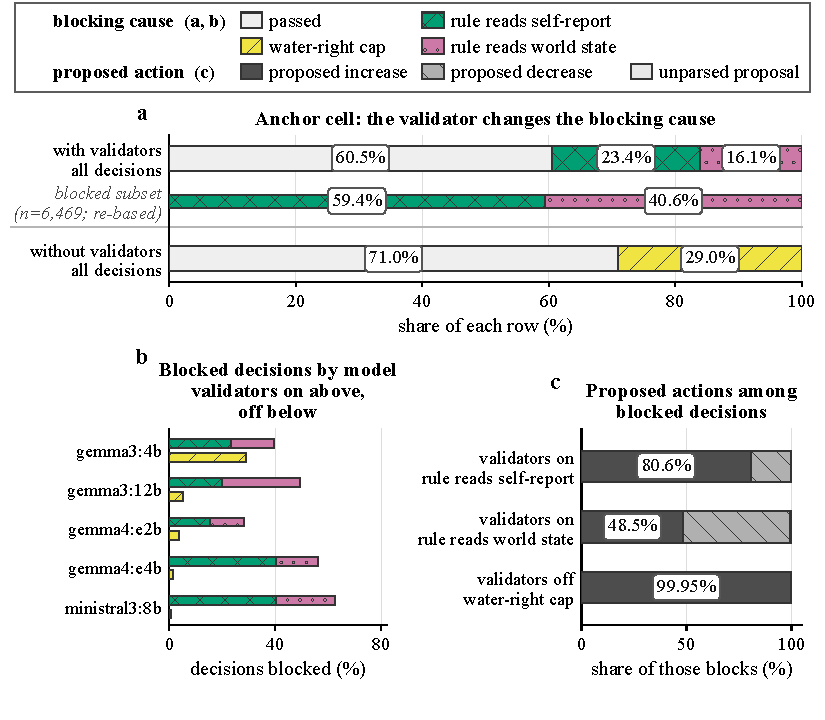
\includegraphics[width=0.8\linewidth]{fig1_rule_layers.pdf}
\caption{Rule-layer decomposition and proposed actions across five LLM configurations in irrigation. \textit{Blocked} means a rejected proposal and \textit{passed} means an approved one. The \textit{water-right cap} is an allocation-cap failure that occurs before any validator rule runs. \textit{Reads self-report} uses an agent-reported condition; \textit{reads world state} uses simulator state only. Panel a is the anchor cell, gemma3:4b, with five seeds. Its outer rows contain all 16,380 decisions per arm. The middle row contains only the 6,469 validator-on rejections and recomputes their shares within that subset; it is not a third arm. Panel b shows the same separation across all five models, exact in 10/10 model-arm cells. Panel c shows proposed actions by blocking rule kind, pooled over the five models. The near-total \textit{proposed increase} share under the water-right cap follows from the configuration, not from behavior (Section 3). \textit{Unparsed proposal} is under half a percent of blocks everywhere and carries no claim. The text uses all validator-on blocks, while panel c uses a separate denominator within each rule type. Counts are pooled across seeds, so this is a decomposition rather than a paired contrast, and no confidence intervals are attached.}
\label{fig:2}
\end{figure}

\section{Enforcement Changes the Reported Condition}
The reported condition changes more than the rate it supports. In the anchor cell, the high-scarcity contrast is +45.73 pp (95\% CI +40.24, +51.21; p < 0.001). The contrast in the conditional increase rate is +23.02 pp (95\% CI +19.06, +26.98; p = 0.0001). High scarcity appears in 37.08\% of governed decisions and 82.80\% of no-validator decisions. Among those decisions, the increase rate is 36.05\% and 59.07\%, respectively. Without prevalence, a changed rate could mean fewer increases, a different set of counted decisions, or both.

The coping report moves too, so scarcity alone does not describe the full rule condition. Coping is reported high in 70.66\% of governed anchor decisions and 83.06\% without validators. The contrast is +12.41 pp (95\% CI +9.78, +15.03). The full conjunction appears in 25.46\% and 68.61\% of the two arms. Its prevalence contrast is +43.15 pp (95\% CI +39.06, +47.24), and its conditional rate gap is +19.86 pp. A second enforced rule, defined by very low reported scarcity on a disjoint set, moves $-$3.27 pp.

The anchor cell is not special. Every irrigation cell moves in the same direction, with contrasts ranging +21.27 pp to +47.53 pp and \textit{p} < 0.05 in all five. The nine flood cells show $-$3.66 to +6.24 pp, mostly null, with five of the nine positive cells and one significant cell (gemma4:26b, +2.92 pp (95\% CI +0.71, +5.12; p = 0.021)). Rejection pressure also differs. Governed irrigation decisions are rejected at 28.09\% to 62.63\% on the Table 1 per-seed- mean basis. Flood pressure ranges 0.00\% to 1.07\%, and the no-validator arm rejects 0.00\%.

We use flood as a portability demonstration, not as a control for enforcement pressure. The regime is confounded with the testbed, and the two testbeds also differ in feedback and reporting instrument. The near-null flood shifts show only that the direction is not universal across the second testbed. They do not isolate a model-family or instrument effect.

\textbf{Table 1.} Agent-reported high-scarcity prevalence and the increase rate among those decisions across fourteen model-testbed cells and both arms. HIGH is the share of decisions whose reported water-scarcity condition is high or very high. It includes every decision satisfying the full two-part rule, plus decisions with low coping. The conditional rate is the share of HIGH decisions whose recorded action was a demand increase; it is not a norm-violation rate. On and off mean with and without validators. Delta is off minus on, so a positive value means that validators lowered the quantity. Cells are per-seed means using \textit{LAST-PROPOSED}, the final proposed action after retries. Each seed contributes one mean (df = \textit{n} - 1). The nine flood cells share one line and carry no conformance rate.

\begin{center}
\small
\setlength{\tabcolsep}{3pt}
\begin{tabular}{llrrrrrrr}
\hline
testbed & model & \textit{n} & HIGH, on & HIGH, off & $\Delta$ HIGH & cond., on & cond., off & $\Delta$ cond. \\
\hline
irrigation & gemma3:4b & 5 & 37.08 & 82.80 & \textbf{+45.73} & 36.05 & 59.07 & \textbf{+23.02} \\
irrigation & gemma3:12b & 3 & 5.49 & 26.76 & \textbf{+21.27} & 5.45 & 16.89 & \textbf{+11.44} \\
irrigation & gemma4:e2b & 5 & 18.26 & 65.79 & \textbf{+47.53} & 12.71 & 31.65 & \textbf{+18.94} \\
irrigation & gemma4:e4b & 5 & 45.27 & 88.65 & \textbf{+43.38} & 23.67 & 41.08 & \textbf{+17.41} \\
irrigation & ministral3:8b & 3 & 13.56 & 44.69 & \textbf{+31.13} & 3.25 & 6.05 & \textbf{+2.80} \\
flood & 9 cells & 5 & --- & --- & $-$3.66 to +6.24 & --- & --- & --- \\
\hline
\end{tabular}
\end{center}

\section{What Recorded-World Reweighting Can and Cannot Show}
On the anchor cell, much of the change in the reported condition follows the arms' different simulator- recorded worlds. The relevant variables---shortage tier, reservoir elevation, and drought index---are written by the simulator rather than by the response being judged. We can therefore use them for a post hoc descriptive comparison. They are independent of the current response, but not independent of enforcement: governance changes the reservoir and therefore the distribution of world states. This analysis is descriptive, not a causal adjustment.

We reweight both arms to the same distribution of recorded world states. The remaining differences are small relative to the raw +45.73 pp gap, but they are not uniformly zero. Reweighting by shortage tier leaves -2.53 pp across 100\% of the anchor corpus. The finest reported stratification leaves +0.21 pp across 43.4\% of the corpus. No reported resolution produces a residual larger than 4.47 pp. These results are consistent with a large composition contribution. They do not show that the agent would give the same report in an identical world.

Table 2 gives the reweighting ladder, with a count and interval at every rung. A stratum enters only if it holds 40 decisions in each arm, so coverage falls as the strata become finer. The finest rung covers just under half of the corpus, and its smallest comparable cell holds 67 decisions. Two of the four intervals exclude zero, both below it. Within those strata, the governed arm reports more scarcity. This is inconsistent with treating the raw shift as purely a reporting effect, but it does not identify a within-world behavioral mechanism.

\textbf{Table 2.} Reported high-scarcity prevalence after stratification on simulator-recorded world state. The anchor cell has five paired seeds and a raw shift of \textbf{+45.73 pp} before reweighting. Residual means no-validator minus with-validators prevalence, in percentage points, after both arms are reweighted to the pooled stratum distribution. Reweighting on either arm's own distribution instead moves the residual by at most 0.78 pp. \textit{n} is the smallest and largest per-arm cell on the rung. The last column recomputes the residual within each seed and gives a paired interval, df = 4. Curtailment ratio is collinear with tier and adds no stratum.

\begin{center}
\small
\setlength{\tabcolsep}{3pt}
\begin{tabular}{lrrrrr}
\hline
recorded-world stratification & strata & n per stratum & coverage & residual & per-seed mean (95\% CI) \\
\hline
shortage tier & 4 & 858--12,558 & 100.0\% & $-$2.53 & $-$3.12 ($-$5.56, $-$0.68) \\
tier + Mead elevation, 25 ft & 7 & 78--4,602 & 81.9\% & $-$4.47 & $-$4.95 ($-$8.29, $-$1.62) \\
tier + Mead 10 ft + drought decile & 19 & 78--1,326 & 50.5\% & +0.57 & $-$0.53 ($-$4.32, +3.25) \\
tier + Mead + drought + agent cluster & 19 & 67--1,139 & 43.4\% & +0.21 & $-$0.87 ($-$4.94, +3.19) \\
\hline
\end{tabular}
\end{center}

The reweighting tracks where each arm spends its run. The governed arm takes 64.8\% of its decisions in shortage tier 0, where no shortage is declared. The no-validator arm takes 76.7\% in tier 3, which represents severe shortage. The two arms therefore occupy different worlds. This comparison does not show that they would produce the same report in an identical world.

The reservoir explains the observed world-state difference (Figure 3b). The governed arm ends +106.57 ft higher on Lake Mead, with an average gap of +102.25 ft over 42 years. The no-validator arm first touches the 895 ft floor in year 17--18 in all five seeds. The governed arm does so in none. This divergence is an observed consequence of the coupled guardrail loop. The data do not identify whether the size of the reporting change scales with the size of the world-state change.

Two further comparisons are consistent with this account. At year 1, the two arms' worlds are identical on all nine pre-decision columns across 390 matched anchor pairs. They first disagree at year 2, and the year-1 prevalence shift is +3.33 pp (95\% CI $-$3.75, +10.42; p = 0.261), a null (Figure 3a). Retry pressure is already high in year 1. 82.1\% of governed year-1 decisions are rejected and retried at least once, compared with 63.8\% across all 42 years. 70.5\% reach the end of the retry budget. The year-1 contrast is not distinguishable from zero. The gap is not monotone after year 1 either: two of the 41 later years run significantly the other way, year 4 at $-$18.46 pp (p = 0.004) and year 7 at $-$6.41 pp (p = 0.001). Years 2 to 11 are mixed in sign. These per-year tests are descriptive checks across correlated years, not multiplicity-adjusted confirmatory claims.

As a descriptive sensitivity check, the never-retried stratum has a larger rather than smaller shift in 5 of 5 irrigation cells (Figure 3c). In the anchor cell, the shift is +53.46 pp, compared with +45.73 pp over all decisions. Pooled over 21 paired seeds, it is +48.21 pp compared with +40.02 pp. This comparison cannot separate world composition from treatment-affected selection because the two arms are filtered differently. The larger contrast is compatible with selection as well as world composition, so it is not evidence that selection is irrelevant. The stratum is also unbalanced: 36.2\% of governed decisions are never retried, compared with 64.6\% of no-validator decisions. One quantity remains unobserved: the reported condition on a governed decision that was retried and then approved. We return to this missing record in Section 8.

% figure source (as recorded in manuscript.md): figures/fig2_mechanism.pdf
\begin{figure}[t]
\centering
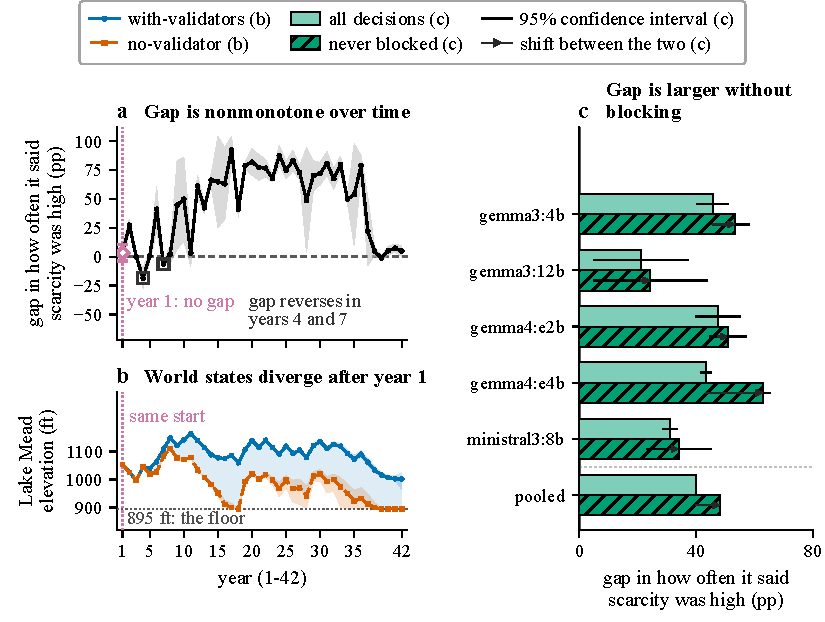
\includegraphics[width=0.8\linewidth]{fig2_mechanism.pdf}
\caption{\textbf{World-state divergence and the agent-reported scarcity gap.} Panels a and c plot the gap in the share of decisions carrying a high or very high agent-reported scarcity condition. The gap is no-validator minus validator-on, in percentage points, so a positive value means that validators lowered the share. \textit{Never blocked} means no rejection, no retry, and retry count zero. \textit{Nonmonotone} means that the gap changes direction over time. Panel a plots the gap by year over 42 simulated years, with a 95\% confidence band across seeds. At year 1 the two arms' worlds are identical on all nine pre-decision columns and the gap is +3.33 pp (p = 0.261), a null. Significant reversals in years 4 and 7 are marked. Panel b plots Lake Mead elevation for each arm, not a gap. Its band is the per-seed min-max range, not a confidence interval. The 895 ft floor is reached by the no-validator arm in every seed and by the governed arm in none. Panel c compares the gap over all decisions with the gap in the never-blocked stratum for five irrigation configurations, pooled over 21 paired seeds. Panels a and b show the anchor cell (gemma3:4b, irrigation), with five paired seeds.}
\label{fig:3}
\end{figure}

\section{Changing the Denominator Changes the Estimate}
Because the reported condition changes, we compare the conditional and fixed-denominator rates. They are different \textit{estimands}, or quantities being estimated. Over 3,276 decisions per run in both arms, the fixed- denominator contrast changes in every irrigation cell. It is smaller in four cells, nearly zero on gemma3:12b, and reverses sign on ministral3:8b (Figure 4).

On the anchor cell, the contrast is +23.02 pp when conditioned on high scarcity. It is +21.62 pp over every decision, a difference of 1.39 pp. The two gemma4 cells also change. gemma4:e2b moves from +18.94 pp to +15.25 pp, and gemma4:e4b moves from +17.41 pp to +8.52 pp.

On gemma3:12b, the conditional contrast changes from +11.44 pp (95\% CI +3.19, +19.69; p = 0.027) to +0.16 pp (95\% CI -13.92, +14.25; p = 0.965) on the \textit{LAST-PROPOSED} action reading used by the reported statistics. If we substitute the executed action on rejected rows, the same fixed-denominator contrast becomes +27.82 pp (p = 0.004). The reported condition changed, but this corpus does not establish a change in the increase rate over a fixed denominator. A reader given only the conditional number could infer a behavior change that this comparison does not identify.

On ministral3:8b, the two statistics disagree in sign: the conditional contrast is +2.80 pp (95\% CI +0.02, +5.58; p = 0.049) versus $-$22.17 pp (95\% CI $-$29.02, $-$15.32; p = 0.005) for the fixed denominator, on three paired seeds at df = 2. Its conditional interval is wider than the effect it brackets and clears zero by less than the second decimal. This supports the reversal between estimands, not the conditional result itself.

A fixed denominator also permits an external reference that the conditional rate cannot use. The irrigation action set holds five skills, two of them increases, so a uniformly random agent would propose an increase on 40\% of decisions. Without validators, the unconditional rate is far above that null (62.52\%, t = 42.66, df = 4, 95\% CI 61.06 to 63.99). With validators, we do not reject comparison with the null (40.90\%, t = 0.46, df = 4, 95\% CI 35.45 to 46.35). No equivalent reference exists for the conditional rate because its denominator is written by the process under evaluation. The null is weak and bounds direction only. A marginal rate at chance means no net pull toward increases, not that governed behavior is random.

% figure source (as recorded in manuscript.md): figures/fig3_consequence.pdf
\begin{figure}[t]
\centering
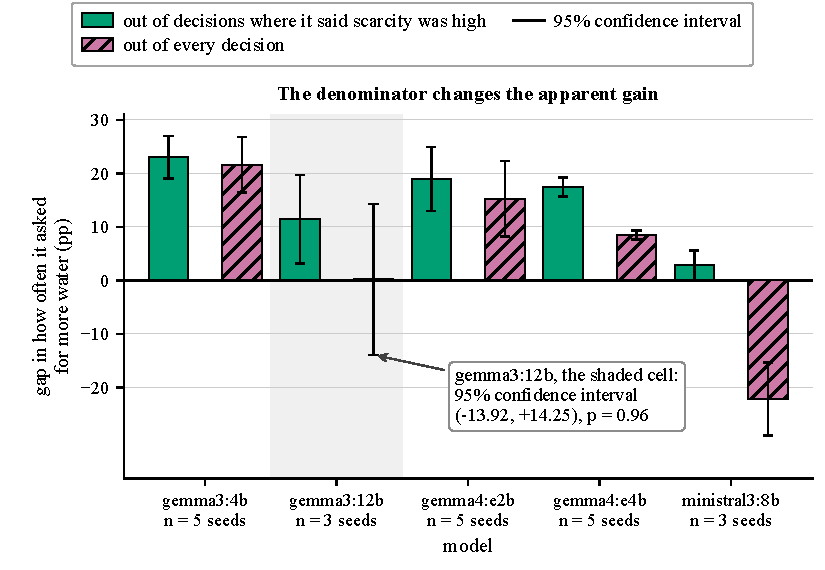
\includegraphics[width=0.8\linewidth]{fig3_consequence.pdf}
\caption{Changing the denominator changes the measured contrast. Each irrigation cell shows two estimates. Solid bars give the rate among decisions where the agent reports high scarcity. Hatched bars give the rate over every decision. The y axis is no-validator minus validator-on, in percentage points, so a positive value means that validators lowered the rate. Whiskers are two-sided 95\% confidence intervals from paired \textit{t}-tests on per-seed gaps, df = \textit{n} - 1. The seed provides one gap per test, and \textit{n} appears under each model. The action reading is \textit{LAST-PROPOSED} throughout. In the shaded gemma3:12b cell, the fixed- denominator estimate is +0.16 pp. Using the executed action on rejected rows moves it to +27.82 pp (p = 0.004). This is an existence proof tied to that action reading, not a general finding. The difference between estimands is descriptive, not causal, and the all-decision rate is not a corrected effect size.}
\label{fig:4}
\end{figure}

\section{Reporting Protocol}
A world-state condition is not an automatic repair. We tested this alternative on the anchor cell. Replacing the agent report with a simulator-recorded condition also changes the counted condition. Shortage tier 2 or worse shifts +64.29 pp against the agent-reported conjunction's +45.73 pp. Tier 1 or worse and a nonzero curtailment ratio each shift +55.71 pp. A drought index at or above 0.5 shifts +25.71 pp. The simulator records these variables outside the response, which makes the reweighting in Section 5 possible. However, governance changes the world through the irrigation feedback loop. The alternative condition is different, not unaffected.

Three reporting requirements follow. First, report the condition's prevalence in both arms beside every conformance rate. Second, log the independent world state behind an agent report when it exists. Third, when the design fixes a denominator, report that all-decision rate beside the conditional rate as a different estimand. Without the world record, a deployment that logs only rule fires, retries, and outcomes cannot recover the descriptive decomposition later.

\section{Limitations and Missing Tests}
An accepted report after a retry is selected by the rule that judged it. This stratum is 24.3\% of governed decisions, and its first attempt is absent from the shipped corpus. Three checks found no first-attempt record. The never-retried stratum is not a bound on this missing quantity. No report there was rewritten, but the two arms are filtered differently.

Finer stratification trades coverage for resolution. The finest rung covers 43.4\%, compared with 100\% for the coarse rung. The corpus covers three open-weight families from 3B to 27B, no frontier models, and flood-only size endpoints. Whether the finding is architectural rather than a capability limit is untested. Regime is confounded with testbed, so inference is within irrigation. One no-validator run used a later code revision and labels the same precondition differently. No rate depends on that label.

Flood has three provenance defects. Denominator coverage is 70.5--100.0\% by design. Manifest seeds disagree in six of the nine flood models when paired by run index. One governed gemma3:4b run used a shorter prompt. None of these defects bears on irrigation.

Two missing data streams would settle the remaining ambiguity. One is the first-attempt report before retry. The other is enforcement with the environment pinned to the untreated trajectory. Neither exists here. This is one guardrail stack with a nondeterministic backend, so comparisons are aggregates over \textit{N} seeds.

\section{Conclusion}
In a guardrail loop with environmental feedback, an agent-reported rule condition can change both the recorded response and the decisions used to score it. Our irrigation results show why a changed conditional rate is not enough to establish a change in the behavior being measured. Report condition prevalence, preserve an independent world-state record, and show an all-decision rate when the design provides one.

\section*{Artifact availability}
On acceptance we will release code, configurations, manifests, and the inventory; one command regenerates tables and figures without GPU or network. Of 42 identifying runs, 27 have enriched and 15 minimal manifests, so dirty or missing hashes prevent clean source-run reproduction for every run. This is a descriptive audit, not a bitwise-reproducible benchmark.

\section*{References}
% BIBLIOGRAPHY:BEGIN -- generated by make_bibliography.py from references.bib; do not hand-edit

[1] Haoyu Wang, Christopher M. Poskitt, and Jun Sun. AgentSpec: Customizable Runtime Enforcement for Safe and Reliable LLM Agents. In Proceedings of the 48th IEEE/ACM International Conference on Software Engineering (ICSE 2026), 2026. arXiv:2503.18666.

[2] Traian Rebedea, Razvan Dinu, Makesh Narsimhan Sreedhar, Christopher Parisien, and Jonathan Cohen. NeMo Guardrails: A Toolkit for Controllable and Safe LLM Applications with Programmable Rails. In Proceedings of the 2023 Conference on Empirical Methods in Natural Language Processing: System Demonstrations, pages 431--445, 2023. Association for Computational Linguistics. doi:10.18653/v1/2023.emnlp-demo.40. arXiv:2310.10501.

[3] Seongjae Kang, Taehyung Yu, and Sung Ju Hwang. PolicyGuard: A Dialogue-Grounded Sub-Agent Verifier for Policy Adherence in LLM Agents. Preprint, 2026. arXiv:2606.29225.

[4] Wenhao Yuan, Chenchen Lin, Jian Chen, Jinfeng Xu, Xuehe Wang, and Edith Cheuk Han Ngai. Verify Before You Commit: Towards Faithful Reasoning in LLM Agents via Self-Auditing. In Proceedings of the 64th Annual Meeting of the Association for Computational Linguistics (ACL 2026), 2026. arXiv:2604.08401.

[5] Davide Grossi, Huib Aldewereld, and Frank Dignum. Ubi Lex, Ibi Poena: Designing Norm Enforcement in E-Institutions. In Coordination, Organizations, Institutions, and Norms in Agent Systems II (COIN 2006, Revised Selected Papers), Lecture Notes in Computer Science, pages 101--114, 2007. Springer. doi:10.1007/978-3-540-74459-7\_7.

[6] Marc Esteva, Bruno Rosell, Juan A. Rodr\'{i}guez-Aguilar, and Josep Llu\'{i}s Arcos. AMELI: An Agent-Based Middleware for Electronic Institutions. In Proceedings of the Third International Joint Conference on Autonomous Agents and Multiagent Systems (AAMAS 2004), pages 236--243, 2004. IEEE Computer Society. doi:10.1109/AAMAS.2004.10060.

[7] Virginia Dignum. A Model for Organizational Interaction: Based on Agents, Founded in Logic. PhD thesis, Utrecht University, 2004. SIKS Dissertation Series. Introduces the OperA model. https://dspace.library.uu.nl/handle/1874/890

[8] Jomi Fred H\"{u}bner, Jaime Sim\~{a}o Sichman, and Olivier Boissier. A Model for the Structural, Functional, and Deontic Specification of Organizations in Multiagent Systems. In Advances in Artificial Intelligence: 16th Brazilian Symposium on Artificial Intelligence (SBIA 2002), Lecture Notes in Computer Science, pages 118--128, 2002. Springer. Introduces the MOISE+ model. doi:10.1007/3-540-36127-8\_12.

[9] Xueping Gao, Jianwei Yang, and Qiang Yang. Looping Is Not Reliability: State-Bound Evidence and Typed Revision Contracts for Agentic Code Repair. Preprint, 2026. arXiv:2607.24604.

[10] Paul R. Rosenbaum. The Consequences of Adjustment for a Concomitant Variable That Has Been Affected by the Treatment. Journal of the Royal Statistical Society, Series A (General), 147(5):656--666, 1984. doi:10.2307/2981697.

[11] Ronald W. Rogers. A Protection Motivation Theory of Fear Appeals and Attitude Change. The Journal of Psychology, 91(1):93--114, 1975. doi:10.1080/00223980.1975.9915803.

[12] Andrew M. Bean and others. Measuring what Matters: Construct Validity in Large Language Model Benchmarks. In 39th Conference on Neural Information Processing Systems (NeurIPS 2025) Track on Datasets and Benchmarks, 2025. arXiv:2511.04703.

[13] Sayash Kapoor, Benedikt Stroebl, Zachary S. Siegel, Nitya Nadgir, and Arvind Narayanan. AI Agents That Matter. Preprint, 2024. arXiv:2407.01502.

[14] Yao Liu, Tien-Ping Tan, and Zhilan Liu. Charge as a Construct-Validity Factor in Chinese Legal Case Retrieval: A Cross-Benchmark Audit. Preprint, 2026. arXiv:2606.12993.

% BIBLIOGRAPHY:END


\end{document}
